\documentclass[12pt]{article}
\usepackage[margin=1in]{geometry}
\usepackage{hyperref}
\usepackage{xurl}
\usepackage{graphicx}
\usepackage{listings}
\usepackage{xcolor}
\usepackage{booktabs}
\usepackage{cite}
\usepackage{subcaption}
\usepackage{tikz}
\usetikzlibrary{arrows.meta,positioning,shapes.geometric}
\usepackage{titlesec}
\titlespacing*{\section}{0pt}{1.2\baselineskip}{0.4\baselineskip}
\setlength{\parskip}{0.4\baselineskip}
\setlength{\parindent}{0pt}

% Allow long /api/... paths and URLs to wrap inside paragraphs.
\usepackage{seqsplit}
\newcommand{\apipath}[1]{\texttt{\seqsplit{#1}}}
\sloppy
\setlength{\emergencystretch}{3em}
\hbadness=10000
\hfuzz=2pt

% Code listing style
\lstset{
  basicstyle=\ttfamily\small,
  backgroundcolor=\color{gray!10},
  frame=single,
  breaklines=true,
  columns=fullflexible,
}

% ── Title block ────────────────────────────────────────────────────────────
\title{
  \textbf{Black-Box Fuzz Testing of the Graylayer Market Proxy API \\
  Using OpenAPI-Guided Test Generation}
}

\author{
  Asray Gopa \and
  Issmale Bekri \and
  Rohan Sah \and
  Akhil Pallem \and
  Peter Collins
}

\date{May 5, 2026}

% ───────────────────────────────────────────────────────────────────────────
\begin{document}

\maketitle

\begin{abstract}
\noindent
We applied schema-guided black-box fuzzing to the production
Graylayer Market Proxy API, a third-party HTTP service that we did
not have source access to. We wrote an OpenAPI 3.0 specification~\cite{openapi_spec}
by hand from the public docs and used it to drive Schemathesis~\cite{schemathesis_paper}
along with three smaller test suites we wrote ourselves: negative,
differential, and stateful. Across 51 endpoints and five upstream
venues, our run recorded 2{,}533 events and turned up 19
high-severity findings. These include two 5xx crashes that we can
reproduce (one on Kalshi markets, one on Gemini trades) and 15
list-then-detail invariant violations on Polymarket and Coinbase
detail endpoints. The rest of this paper walks through what
schema-guided fuzzing caught, what it missed, and where we think it
fits in a wider API testing strategy.
\end{abstract}

% ───────────────────────────────────────────────────────────────────────────
\section{Introduction}
\label{sec:intro}

\noindent
Modern web services expose large attack surfaces through their APIs.
When developers write manual tests, there are only limited amounts of
inputs to try. This leaves a lot of edge cases untested, like weird
boundary values, missing fields, or malformed data. Fuzzing is a
testing technique that helps solve this problem by automatically
generating many different inputs and sending them to a program to
see if anything breaks.

\noindent
In this project, we applied fuzzing to the Graylayer Market Proxy
API~\cite{graylayer_docs}, which is a service that pulls together
market data from Polymarket, Kalshi, Gemini, Coinbase, and
Forecastex. Since we do not have access to the source code, we treat
it as a black box. We first wrote an OpenAPI 3.0~\cite{openapi_spec}
specification based on the published documentation, then used that spec to drive four
types of tests: schema-guided fuzzing with
Schemathesis~\cite{schemathesis_docs}, hand-written negative inputs,
differential tests that check cross-endpoint properties, and stateful
tests that verify list-then-detail flows. The goal is to find
crashes, bad error handling, and any behavior that does not match
what the API is supposed to do.

% ───────────────────────────────────────────────────────────────────────────
\section{Previous and Existing Approaches}
\label{sec:prev}

\noindent
Before fuzzing, several techniques were used to find software vulnerabilities and robustness failures. Manual code inspections were the earliest approaches. A human code reviewer would read sections of a codebase or changes made and attempt to identify unexpected or dangerous code patterns. Although a seasoned engineer may be able to provide feedback that causes positive changes, manual reviews are tedious, time consuming, and highly prone to human error. A related technique, penetration testing, had security experts review code with a specific focus on identifying exploitable vulnerabilities. While more targeted than general code review, penetration testing has the same scaling problem. Skilled security testers are expensive and specialized, and they cannot realistically cover every code path in a large system~\cite{godefroid_fuzzing}.

\noindent
Static code analyzers were another common technique, which are automated tools used to identify potentially dangerous code and coding practices. The entire codebase is searched for suspect patterns and dangerous functions that could indicate potential vulnerabilities~\cite{godefroid_fuzzing}. The main downside of these tools is that they are blind at runtime. They cannot detect errors that only show up while a program is running, such as memory corruption under specific conditions.

\noindent
Black-box techniques like Boundary Value Analysis (BVA) are also used to detect errors. BVA aims to test the boundaries between equivalence classes defined in the input domain, and is effective at identifying edge cases in certain scenarios~\cite{acar_bva}. However, it struggles when combinatorial effects of related inputs cause unexpected behavior, and its effectiveness depends on accurate input specifications.

\noindent
Fuzzing itself has gone through a few generations. The original 1990 study by Miller et al.\ used purely random byte streams to crash UNIX utilities~\cite{miller_fuzzing}, and it showed that even unstructured input can uncover real bugs. Coverage-guided fuzzers like AFL~\cite{afl} and AFLplusplus added instrumentation feedback, so mutation could pick inputs that exercise new code paths. This worked well on binaries where source or recompilation is available. Schema-guided API fuzzers like Schemathesis are a third point on this spectrum: they give up source-level coverage feedback in exchange for a structured input model built from an OpenAPI spec. That tradeoff is the only practical one when the system under test is a remote service that you can only reach over HTTP.

\noindent
All of the older techniques rely on human intuition and domain knowledge to decide which inputs or coding patterns to look for. Fuzzing addresses this directly by generating inputs at a much larger scale than any human can, which removes the human bottleneck and the need for someone to know the system in detail beforehand.

% ───────────────────────────────────────────────────────────────────────────
\section{Technical Description}
\label{sec:tech}

\noindent
Schemathesis is a schema-guided API fuzzer built on top of the
Hypothesis property-based testing library~\cite{hypothesis_docs}.
It reads an OpenAPI specification and uses it to automatically
generate and send HTTP requests, then checks the
responses for crashes, invalid JSON, and slow responses. Since
we have no access to the Graylayer source code, we use
\texttt{market\_proxy.yaml} to guide what inputs the fuzzer generates.
Figure~\ref{fig:flow} summarizes the pipeline.

\begin{figure}[h]
\centering
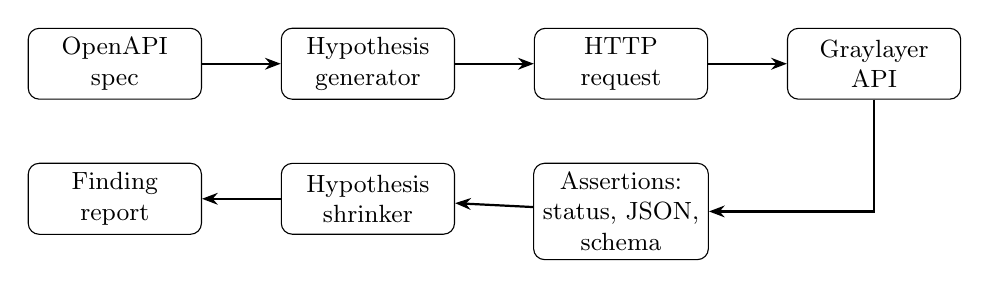
\begin{tikzpicture}[
  node distance=8mm and 10mm,
  box/.style={rectangle, draw, rounded corners, align=center,
              minimum height=9mm, minimum width=22mm, font=\small},
  arr/.style={-{Stealth[length=2mm]}, thick}
]
\node[box] (spec)   {OpenAPI\\spec};
\node[box, right=of spec] (hyp) {Hypothesis\\generator};
\node[box, right=of hyp]  (req) {HTTP\\request};
\node[box, right=of req]  (api) {Graylayer\\API};
\node[box, below=of req]  (chk) {Assertions:\\status, JSON,\\schema};
\node[box, below=of hyp]  (shr) {Hypothesis\\shrinker};
\node[box, below=of spec] (rep) {Finding\\report};
\draw[arr] (spec) -- (hyp);
\draw[arr] (hyp)  -- (req);
\draw[arr] (req)  -- (api);
\draw[arr] (api)  |- (chk);
\draw[arr] (chk)  -- (shr);
\draw[arr] (shr)  -- (rep);
\end{tikzpicture}
\caption{Schema-guided fuzzing pipeline. The OpenAPI spec constrains
input generation; failed assertions feed back into Hypothesis's
shrinker, which produces a minimal reproducer.}
\label{fig:flow}
\end{figure}

\noindent
Before fuzzing begins, Schemathesis reads
\texttt{market\_proxy.yaml} and parses every endpoint, HTTP
method, parameter type, and response schema inside it. This
gives the fuzzer a complete map of the API so it knows what valid
inputs look like for each endpoint.

\noindent
After loading the spec, the fuzzing works as follows:

\begin{enumerate}
  \item Read the OpenAPI spec and collect all operations, which are
  each combination of an endpoint and an HTTP method.
  \item For each operation, use Hypothesis to generate many varied
  inputs based on the declared parameter types, constraints, and
  enums.
  \item Assemble each generated input into a complete HTTP request
  and send it to the live API with our API key.
  \item Check the response against three assertions: the status
  code must not be a server crash, the body must be
  valid JSON if the Content-Type says so, and the response must
  not take longer than 10 seconds.
  \item If any assertion fails, Hypothesis shrinks the input down
  to the smallest version that still causes the failure.
  \item Move to the next operation and repeat.
\end{enumerate}

\noindent
We can walk through an example using the
\apipath{GET /api/v1/kalshi/markets} endpoint from our
\texttt{market\_proxy.yaml}. The relevant slice of that spec is:

\begin{lstlisting}[language=]
/api/v1/kalshi/markets:
  get:
    operationId: kalshiListMarkets
    parameters:
      - name: limit
        in: query
        schema: { type: integer, minimum: 1, maximum: 1000 }
      - name: status
        in: query
        schema: { type: string, enum: [open, closed, settled] }
      - name: min_close_ts
        in: query
        schema: { type: integer, format: int64 }
    responses:
      "200": { description: Market list }
      "400": { description: Bad request }
      "502": { description: Upstream error }
\end{lstlisting}

\noindent
This declares a \texttt{limit} parameter as an integer with
\texttt{minimum: 1} and \texttt{maximum: 1000}.

\begin{enumerate}
  \item Read the spec. The \texttt{limit} parameter is identified
  as an integer with minimum 1 and maximum 1000.

  \item Hypothesis generates test inputs. Say it generates
  \texttt{limit=100}, \texttt{limit=0}, \texttt{limit=-1}, and
  \texttt{limit=1001}. Schemathesis will normally generate many
  more, but for this example, we will use four.

  \item Each input is assembled into a real HTTP GET request and
  sent to the live Graylayer endpoint with our API key.

  \item The responses are checked. \texttt{limit=100} returns 200
  and passes all three assertions. \texttt{limit=0} and
  \texttt{limit=-1} are below the declared minimum so the server
  should return a 4xx rejection. \texttt{limit=1001} is above the
  declared maximum and should also be rejected. If any of these
  return a 500 error, the assertion below fails, and the case
  is flagged:

\begin{lstlisting}[language=Python]
assert response.status_code < 500, (
    f"SERVER ERROR\n"
    f"  Endpoint : {case.method} {case.path}\n"
    f"  Status   : {response.status_code}\n"
    f"  Query    : {case.query}\n"
    f"  Body     : {response.text[:500]}"
)
\end{lstlisting}

  \item If a failure is found, Hypothesis shrinks the input. For
  example if \texttt{limit=-999} caused a 500 error, Hypothesis
  would try \texttt{limit=-1} and confirm that is the smallest
  input that still fails.

  \item Move to the next operation and repeat.
\end{enumerate}

\noindent
On top of Schemathesis we also wrote three smaller test suites that
share the same spec but each ask a different question.
\emph{Negative} tests send malformed inputs by hand, including null
bytes, oversized strings, and out-of-range numbers, to check how the
API handles inputs that the spec explicitly forbids.
\emph{Differential} tests look at cross-endpoint properties, for
example whether two endpoints that should return the same field
actually agree. \emph{Stateful} tests check multi-call flows: every
market ID returned by a list endpoint must also be fetchable from
the matching detail endpoint. The four suites together cover much
more than any single one of them does on its own.

% ───────────────────────────────────────────────────────────────────────────
\section{Evaluation}
\label{sec:eval}

\noindent
To evaluate the technique from Section~\ref{sec:tech} we ran all
four test suites against the production Graylayer Market Proxy
gateway. We wrote one \texttt{market\_proxy.yaml} file from the
public docs, which gave the fuzzer a map of 51 unique operations
covering the Coinbase, Polymarket, Kalshi, Gemini, and Forecastex
venues. We ran the Schemathesis suite from its command-line tool,
with our custom \texttt{no\_5xx\_except\_upstream} check enabled, an
\texttt{X-API-Key} header attached to every request, and a
per-operation example budget set through Hypothesis's
\texttt{max\_examples} option. The negative, differential, and
stateful suites are plain \texttt{pytest} cases under
\texttt{tests/}. We logged every response to JSON Lines files in
\texttt{results/} so we could replay and inspect individual events
later.

\begin{table}[h]
\centering
\small
\begin{tabular}{lrrl}
\toprule
Suite        & Events & High-severity & Notable findings \\
\midrule
Schemathesis & 2{,}484 & 3  & 1 crash, 2 contract violations \\
Negative     & 34      & 1  & 1 crash on Gemini trades \\
Stateful     & 15      & 15 & list/detail invariant breaks \\
Differential & 0       & 0  & all properties held \\
\midrule
Total        & 2{,}533 & 19 & \\
\bottomrule
\end{tabular}
\caption{Findings by test suite.}
\label{tab:summary}
\end{table}

\noindent
Across all four suites we recorded 2{,}533 events. We define an
``event'' as a single generated request together with the result of
the suite's assertions. Of these, 19 were classified as
high-severity, 6 as low, 1{,}339 as medium, and 1{,}169 as
informational (Figure~\ref{fig:overview}). Schemathesis produced
most of the volume, but the stateful suite had the highest hit rate:
all 15 of its events were high-severity.

\begin{figure}[htbp]
\centering
\begin{subfigure}{0.48\textwidth}
  \centering
  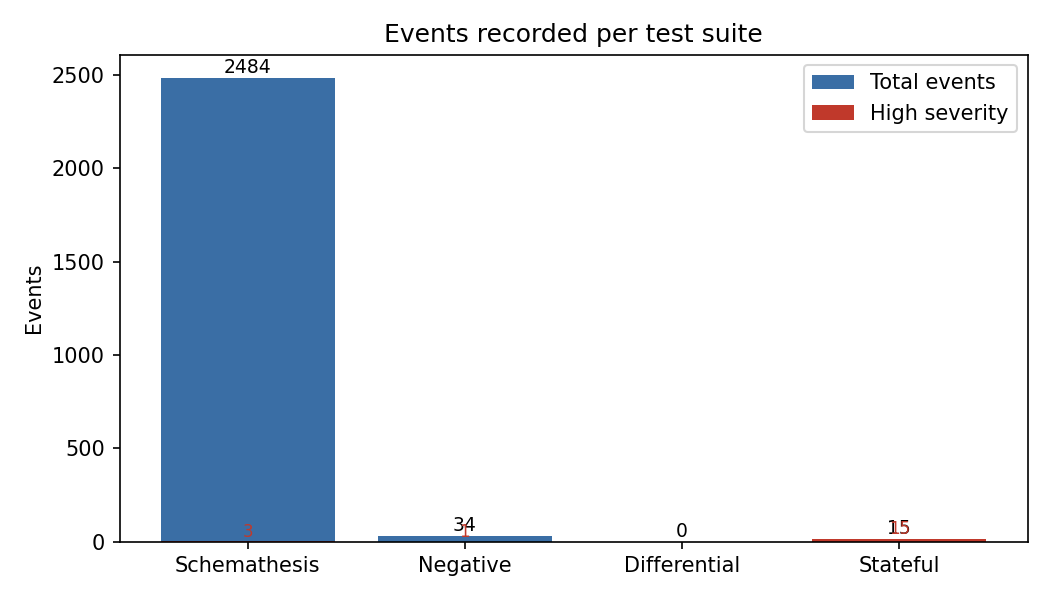
\includegraphics[width=\linewidth]{../results/by_suite.png}
  \caption{Events per test suite. The red overlay marks high-severity findings.}
  \label{fig:suite}
\end{subfigure}\hfill
\begin{subfigure}{0.48\textwidth}
  \centering
  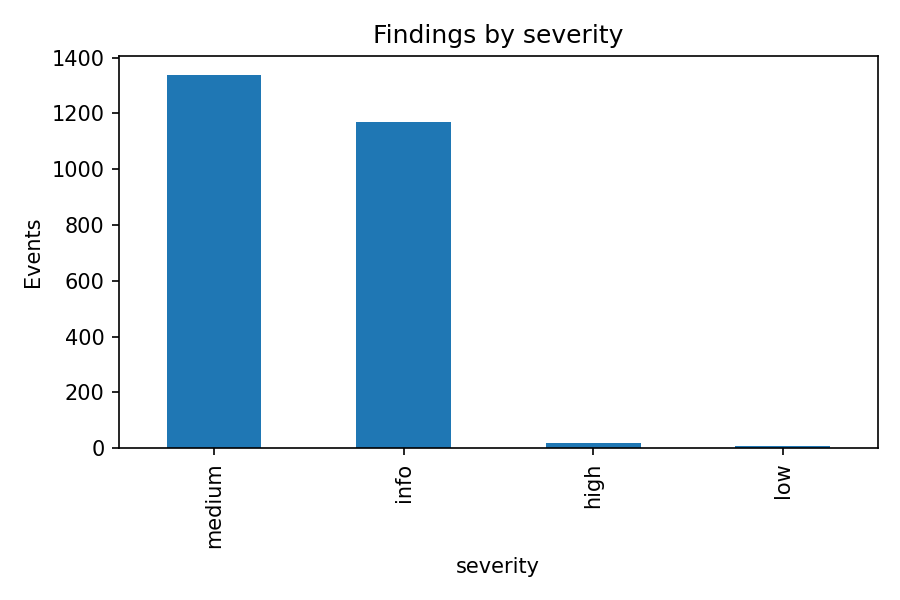
\includegraphics[width=\linewidth]{../results/by_severity.png}
  \caption{Events grouped by severity tier.}
  \label{fig:sev}
\end{subfigure}
\caption{Overall event distribution across the 2{,}533-event run.}
\label{fig:overview}
\end{figure}

\noindent
The two most serious crashes came from different suites and hit
different parts of the gateway. Schemathesis got an HTTP 500 out of
\apipath{GET /api/v1/kalshi/markets} when Hypothesis combined a
\texttt{limit} value of 443 with cursor and ticker parameters that
contained high-bit Unicode characters. The server returned an
\texttt{internal\_server\_error} from the \texttt{query-exchange}
service instead of a 4xx validation error. The negative suite got a
second HTTP 500 out of \apipath{GET /api/v1/gemini/v1/trades/BTCUSD}
when we sent the \texttt{limit\_trades} query parameter as the
literal string \texttt{"many"}. The upstream Gemini service
responded with a generic \texttt{InternalServerError} instead of
the gateway rejecting the malformed input at the proxy layer. These
are the kind of weird inputs a hand-written test suite would never
think to try, and we found them without any instrumentation of the
target service. Figure~\ref{fig:high} ranks every high-severity
endpoint by how many findings it produced.

The shrunken Kalshi reproducer that Hypothesis captured is short
enough to file as a bug report:

\begin{lstlisting}[basicstyle=\ttfamily\scriptsize]
curl -X GET \
  -H 'X-API-Key: ...' \
  -H 'Accept: application/json' \
  'https://gateway.graylayer.tech/api/v1/kalshi/markets?limit=443\
&event_ticker=%C2%A86kv%C2%BB%C2%BD%14%C3%9F\
&series_ticker=y+%C3%B8%C2%86%F4%8F%BA%98%C2%88E\
&max_close_ts=5852907872421506007\
&min_close_ts=-28971\
&cursor=%C3%B1%C3%9D%C3%99%F1%A1%88%85'

# Response: 500
# {"error":{"code":"internal_server_error",
#           "service":"query-exchange"}}
\end{lstlisting}

\begin{figure}[htbp]
\centering
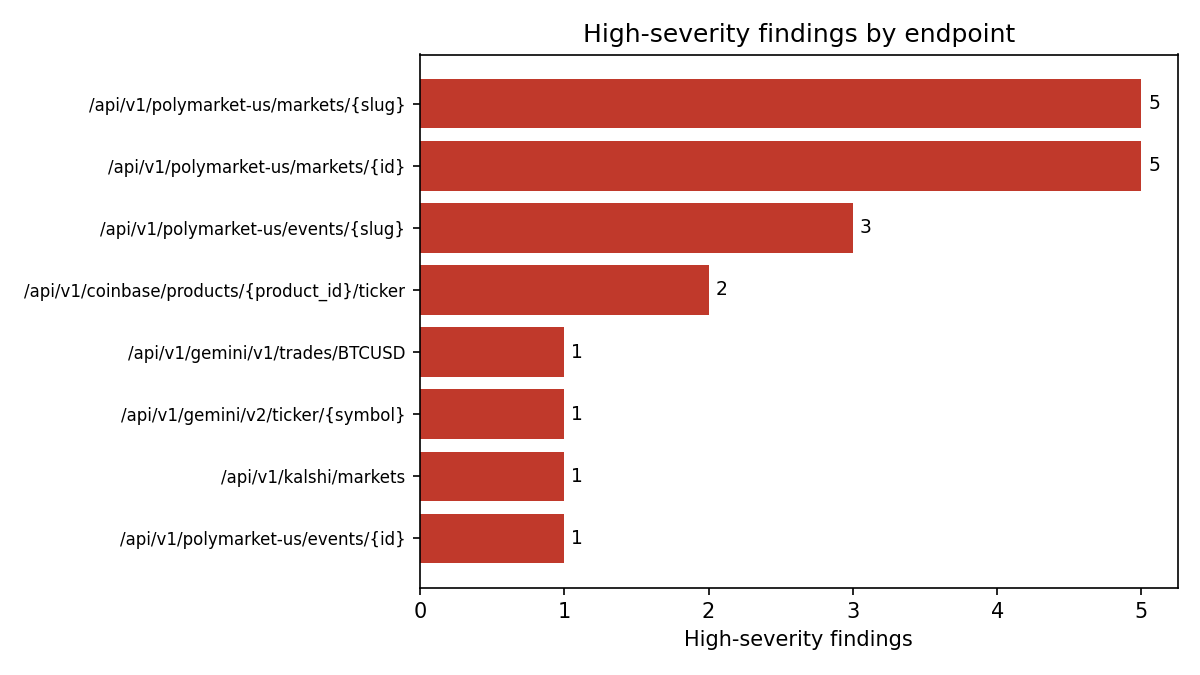
\includegraphics[width=0.75\textwidth]{../results/high_by_endpoint.png}
\caption{High-severity findings by endpoint. The Polymarket
list-then-detail invariant breaks dominate; the two 5xx crashes
appear on \texttt{/kalshi/markets} and \texttt{/gemini/v1/trades/BTCUSD}.}
\label{fig:high}
\end{figure}

\noindent
The stateful suite found a different and arguably more interesting
class of bug: 15 list-then-detail invariant violations, mostly on
\apipath{/api/v1/polymarket-us/markets/\{id\}} (5 cases),
\apipath{/api/v1/polymarket-us/markets/\{slug\}} (5 cases),
\apipath{/api/v1/polymarket-us/events/\{slug\}} (3 cases), and
\apipath{/api/v1/coinbase/products/\{product\_id\}/ticker} (2 cases).
In each case our test took an ID returned by the list endpoint and
immediately requested the matching detail endpoint, and the gateway
responded with a 404. This either means there is some eventual
consistency between the list and detail backends or there is a
routing rule that drops valid IDs. Either way, it is the type of
cross-endpoint bug that single-request fuzzers cannot find. The
differential suite recorded zero findings, which is itself useful
evidence: the five cross-endpoint properties we encoded all held
across this run. Those properties were (1) every documented platform
(Polymarket, Kalshi, Coinbase, Gemini, Forecastex) is reachable
through the gateway and does not return ``Unknown platform'';
(2) Polymarket order books are never crossed, meaning the best bid
is always less than or equal to the best ask; (3) Gemini order
books are never crossed; (4) Kalshi pagination is monotone, so
successive cursors do not revisit IDs; and (5) the authentication
gate is consistent, so requests with no key and requests with a bad
key both return 401 with the same body shape.

\begin{figure}[htbp]
\centering
\begin{subfigure}{0.48\textwidth}
  \centering
  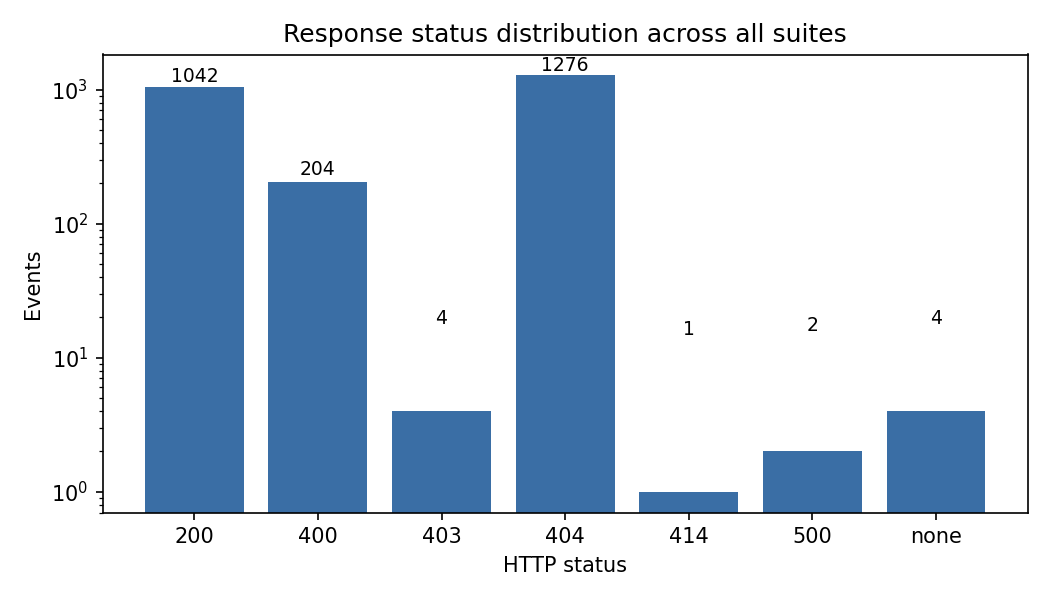
\includegraphics[width=\linewidth]{../results/by_status.png}
  \caption{HTTP response status distribution (log scale).
  The two 500s correspond to the crashes discussed above.}
  \label{fig:status}
\end{subfigure}\hfill
\begin{subfigure}{0.48\textwidth}
  \centering
  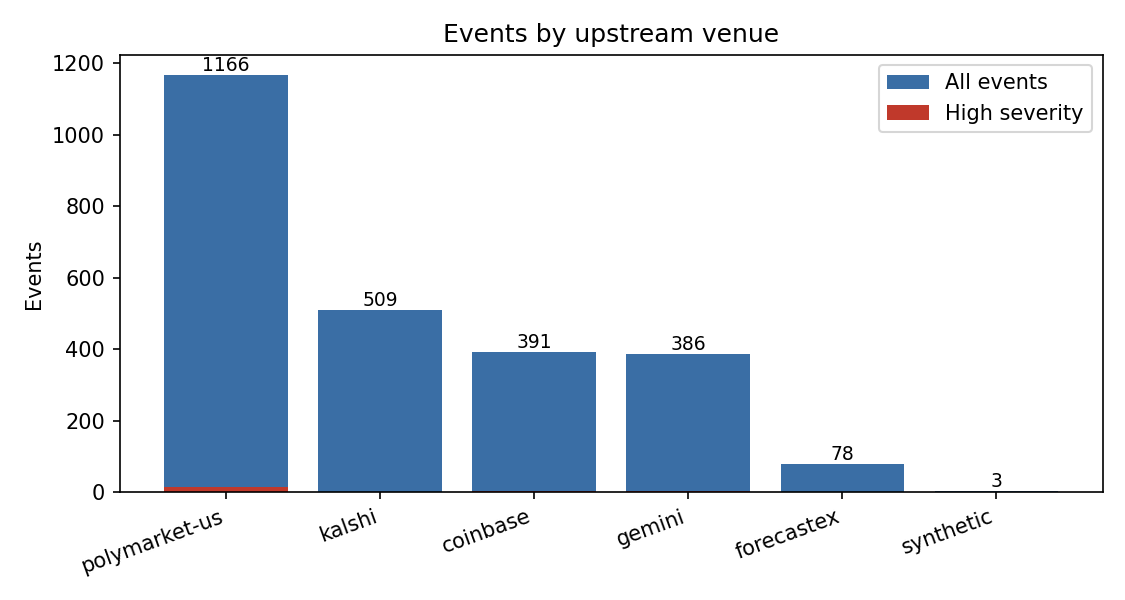
\includegraphics[width=\linewidth]{../results/by_venue.png}
  \caption{Events per upstream venue. Polymarket dominates the volume
  and accounts for most high-severity findings.}
  \label{fig:venue}
\end{subfigure}
\caption{Response and venue distributions.}
\label{fig:dist}
\end{figure}

\noindent
The rest of the unexpected events fell into two big buckets. About
114 events were transport-layer failures, mostly read timeouts and
TCP resets clustered around the higher-volume Polymarket history
endpoints under sustained load. Another 1{,}224 events were tagged
\texttt{unexpected}: status codes that are technically reasonable
(429 rate limits, 414 URI-too-long) but that the spec did not list
as possible responses, so Schemathesis flagged them as schema
contract violations. Two more events were high-severity contract
violations: an undocumented 400 from
\apipath{GET /api/v1/polymarket-us/events/\{id\}} when the path
parameter was non-numeric, and an undocumented 400 from
\apipath{GET /api/v1/gemini/v2/ticker/\{symbol\}} for an unknown
symbol. The total status code distribution was 1{,}042 \texttt{200},
1{,}276 \texttt{404}, 204 \texttt{400}, 4 \texttt{403}, 1
\texttt{414}, and 2 \texttt{500}.

\noindent
We set the example budget per-operation rather than globally, and
several operations stopped early once they hit their first failure.
That is why the total event count of 2{,}533 is below the naive
ceiling of 51 operations times the configured example budget.
Figure~\ref{fig:nonok} shows the per-endpoint non-OK volume; the
flat plateau at the top reflects the per-operation cap, not a
saturating bug rate.

\begin{figure}[htbp]
\centering
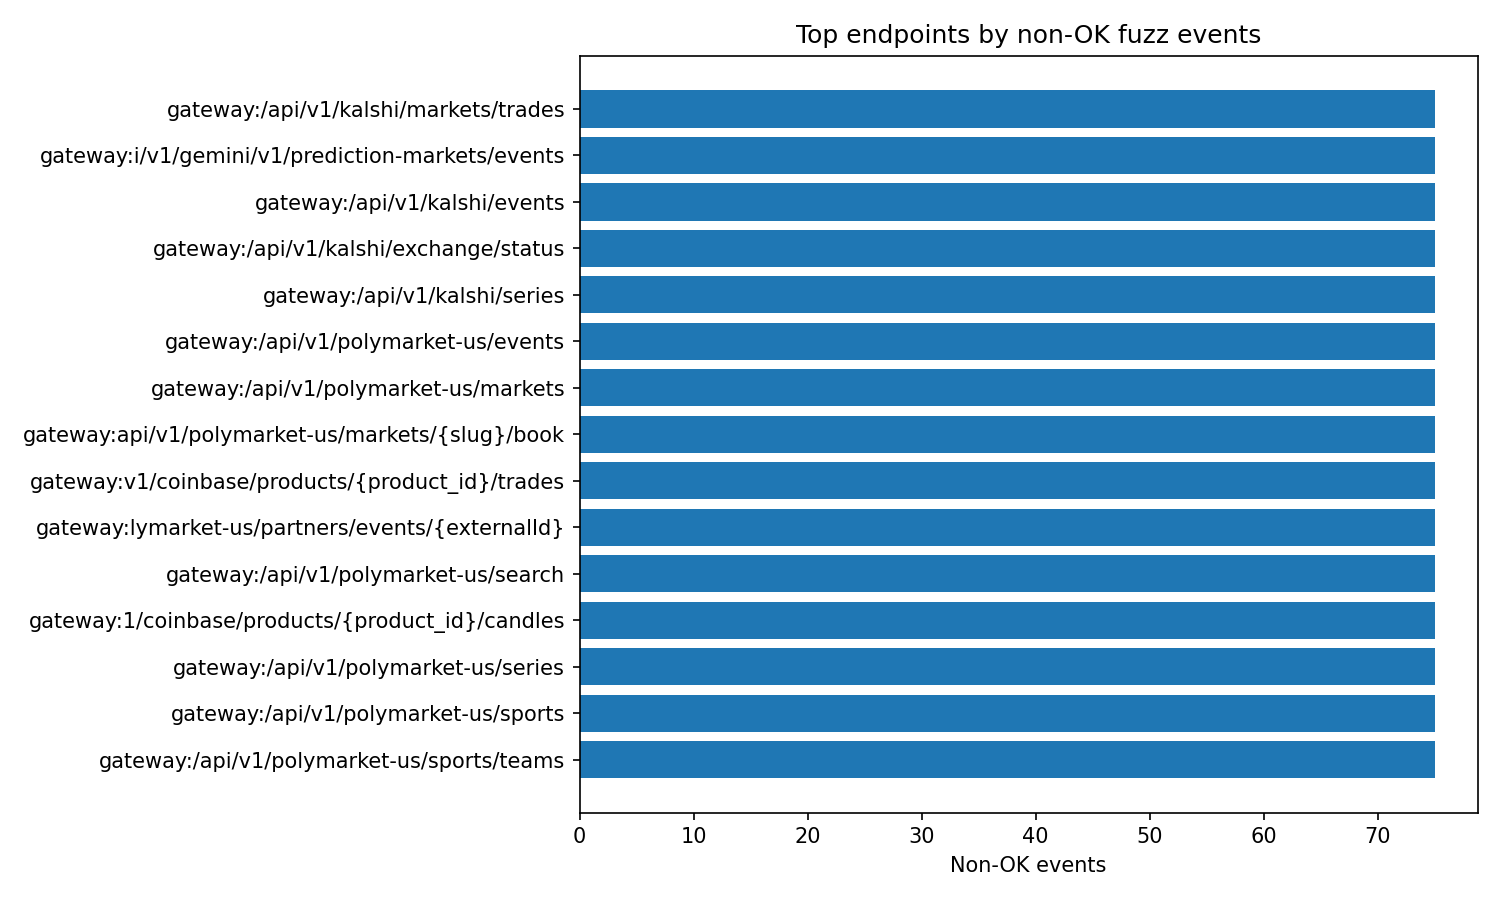
\includegraphics[width=0.85\textwidth]{../results/by_endpoint.png}
\caption{Top endpoints by non-OK fuzz events. The uniform 75-event
height is an artifact of the per-operation example cap, not a
property of the underlying service.}
\label{fig:nonok}
\end{figure}

\subsection*{Threats to validity}

\noindent
A few limitations are worth noting before reading too much into the
numbers above. First, we wrote the OpenAPI spec by hand from the
public docs, so it almost certainly does not match the live
implementation in every place. Some of the 1{,}224 ``unexpected''
status events probably reflect gaps in our spec rather than real
bugs in the service. Second, this is a single run against a
production service whose state changes minute to minute. List
endpoints return different IDs across runs, so the exact stateful
invariant counts are not deterministic, though the underlying
list/detail mismatch on Polymarket was stable across every run we
tried. Third, we only exercised endpoints reachable with one API
key, so authenticated and write-side flows were out of scope.
Fourth, the per-operation example budget was small enough that some
operations probably still have crashes we did not reach. Finally,
transient network errors (the 114 transport events) inflate the
unexpected-event total without pointing to any real bug in the
gateway logic.

\noindent
The advantages of this technique were obvious right away. With no
access to the Graylayer source and only a hand-written spec, we
generated several thousand request/response pairs and isolated two
reproducible 5xx crashes plus 17 other high-severity bugs in under
an hour of wall time. Hypothesis's shrinking gave us a minimal
failing input for every Schemathesis bug, which makes writing up a
report easy. The main disadvantage is that coverage is bounded by
the spec. Any endpoint, parameter, or response field that is missing
from \texttt{market\_proxy.yaml} is invisible to the fuzzer. Stateful
flows that need more setup than a single list-then-fetch (for
example, creating a session token before reading user-scoped data)
also need extra hooks. So we think schema-guided fuzzing is best
seen as a low-effort first pass for any third-party API where you
do not have source access. It finds crashes and contract drift
fast, but it should be paired with hand-written stateful tests and
human review before anyone calls the system safe.

% ───────────────────────────────────────────────────────────────────────────
\section{Summary and Recommendation}
\label{sec:summary}

\noindent
In this project we evaluated schema-guided black-box API fuzzing
on the production Graylayer Market Proxy gateway, using
Schemathesis along with our own negative, differential, and
stateful test suites. We exercised 51 endpoints and recorded
2{,}533 events. Schemathesis found one 5xx crash on
\apipath{/api/v1/kalshi/markets} and two undocumented 4xx contract
violations. The negative suite found one 5xx crash on the Gemini
trades endpoint. The stateful suite found 15 list-then-detail
invariant violations on Polymarket and Coinbase detail endpoints.
The differential suite passed clean. Together the four suites
produced 19 high-severity findings, which shows that even a
well-documented public API can have bugs that manual testing would
not reach.

\noindent
Schema-guided fuzzing turned out to be a good way to find server
crashes, schema drift, and undocumented status codes, and it took
very little manual effort beyond writing the OpenAPI spec. Its
coverage is bounded by the accuracy of that spec: any behavior not
described in the YAML is invisible to the fuzzer. That is the core
limitation of any black-box approach. Based on this, we recommend
this technique for robustness and contract checks of third-party
APIs where you do not have source access, and as a low-effort first
pass before manual penetration testing or authenticated end-to-end
tests. To build a stronger testing lifecycle it should be paired
with stateful suites (which found the highest-impact findings in
our run), static schema linting, and a manual review of the crash
cases we identified.

\noindent
\textbf{Future work.} There are three obvious next steps. First,
adding authentication hooks would let the fuzzer exercise the
write-side and user-scoped endpoints we left out. Schemathesis
supports per-operation auth providers, so this is mostly a
configuration change. Second, running the harness in CI as a
nightly job, with an allowlist of known schema drifts, would turn
these one-shot findings into a regression signal that catches future
contract breaks as soon as they ship. Third, the stateful suite
could be extended from list-then-detail to arbitrary OpenAPI
\texttt{links} chains. That would let it cover multi-step flows
(for example, search then market then orderbook) that the current
single-hop check cannot reach.

% ───────────────────────────────────────────────────────────────────────────
\bibliographystyle{IEEEtran}
\begin{thebibliography}{9}

\bibitem{graylayer_docs}
Graylayer, ``Graylayer API Documentation,''
\url{https://docs.graylayer.tech}, accessed Apr.\ 2026.

\bibitem{schemathesis_docs}
Schemathesis Contributors, ``Schemathesis: Property-Based Testing for API Schemas,''
\url{https://schemathesis.readthedocs.io}, accessed Apr.\ 2026.

\bibitem{hypothesis_docs}
D. R. MacIver \textit{et al.}, ``Hypothesis: A new approach to property-based testing,''
\textit{Journal of Open Source Software}, vol.\ 4, no.\ 43, p.\ 1891, 2019.

\bibitem{fuzzing_usenix}
A. Gutmann, ``Fuzzing: The state of the art,''
\textit{USENIX ;login:}, vol.\ 41, no.\ 2, 2016.
[Online]. Available: \url{https://www.usenix.org/system/files/login/articles/login_summer16_03_gutmann.pdf}

\bibitem{afl}
M. Zalewski, ``American Fuzzy Lop (AFL),''
\url{https://github.com/google/AFL}, accessed Apr.\ 2026.

\bibitem{godefroid_fuzzing}
P. Godefroid, ``Fuzzing,''
\textit{Communications of the ACM}, vol.\ 66, no.\ 9, 2023.
[Online]. Available: \url{https://cacm.acm.org/research/fuzzing/}

\bibitem{acar_bva}
G. Acar, ``Unleashing the Power of Equivalence Partitioning and Boundary Value Analysis in Software Testing,''
\url{https://www.commencis.com/thoughts/unleashing-the-power-of-equivalence-partitioning-and-boundary-value-analysis-in-software-testing/}, accessed May 2026.

\bibitem{miller_fuzzing}
B. P. Miller, L. Fredriksen, and B. So, ``An empirical study of the reliability of UNIX utilities,''
\textit{Communications of the ACM}, vol.\ 33, no.\ 12, pp.\ 32--44, 1990.

\bibitem{schemathesis_paper}
Z. Hatfield-Dodds and D.~R. MacIver, ``Deriving semantics-aware fuzzers from web API schemas,''
in \textit{Proc.\ 44th Int.\ Conf.\ Software Engineering: Companion Proceedings (ICSE-Companion)},
2022, pp.\ 345--346.
[Online]. Available: \url{https://doi.org/10.1145/3510454.3528637}

\bibitem{openapi_spec}
OpenAPI Initiative, ``OpenAPI Specification v3.0.3,''
\url{https://spec.openapis.org/oas/v3.0.3}, accessed Apr.\ 2026.

\end{thebibliography}

\end{document}
